% ============================================================
% Chapter IV — Results and Discussion
% ============================================================
\section{Results and Discussion}

This chapter presents the findings from the multivariate statistical analyses
and machine learning validation. Results are organized sequentially: first the
assumption tests that guided method selection, then the primary inferential
model, and finally the cross-validation outcomes.

\subsection{Descriptive Statistics}

The processed dataset contains 2,880 lap-level observations distributed across
three finishing tiers. Figure~\ref{fig:class-dist} shows the class
distribution.

\begin{figure}[htbp]
  \centering
  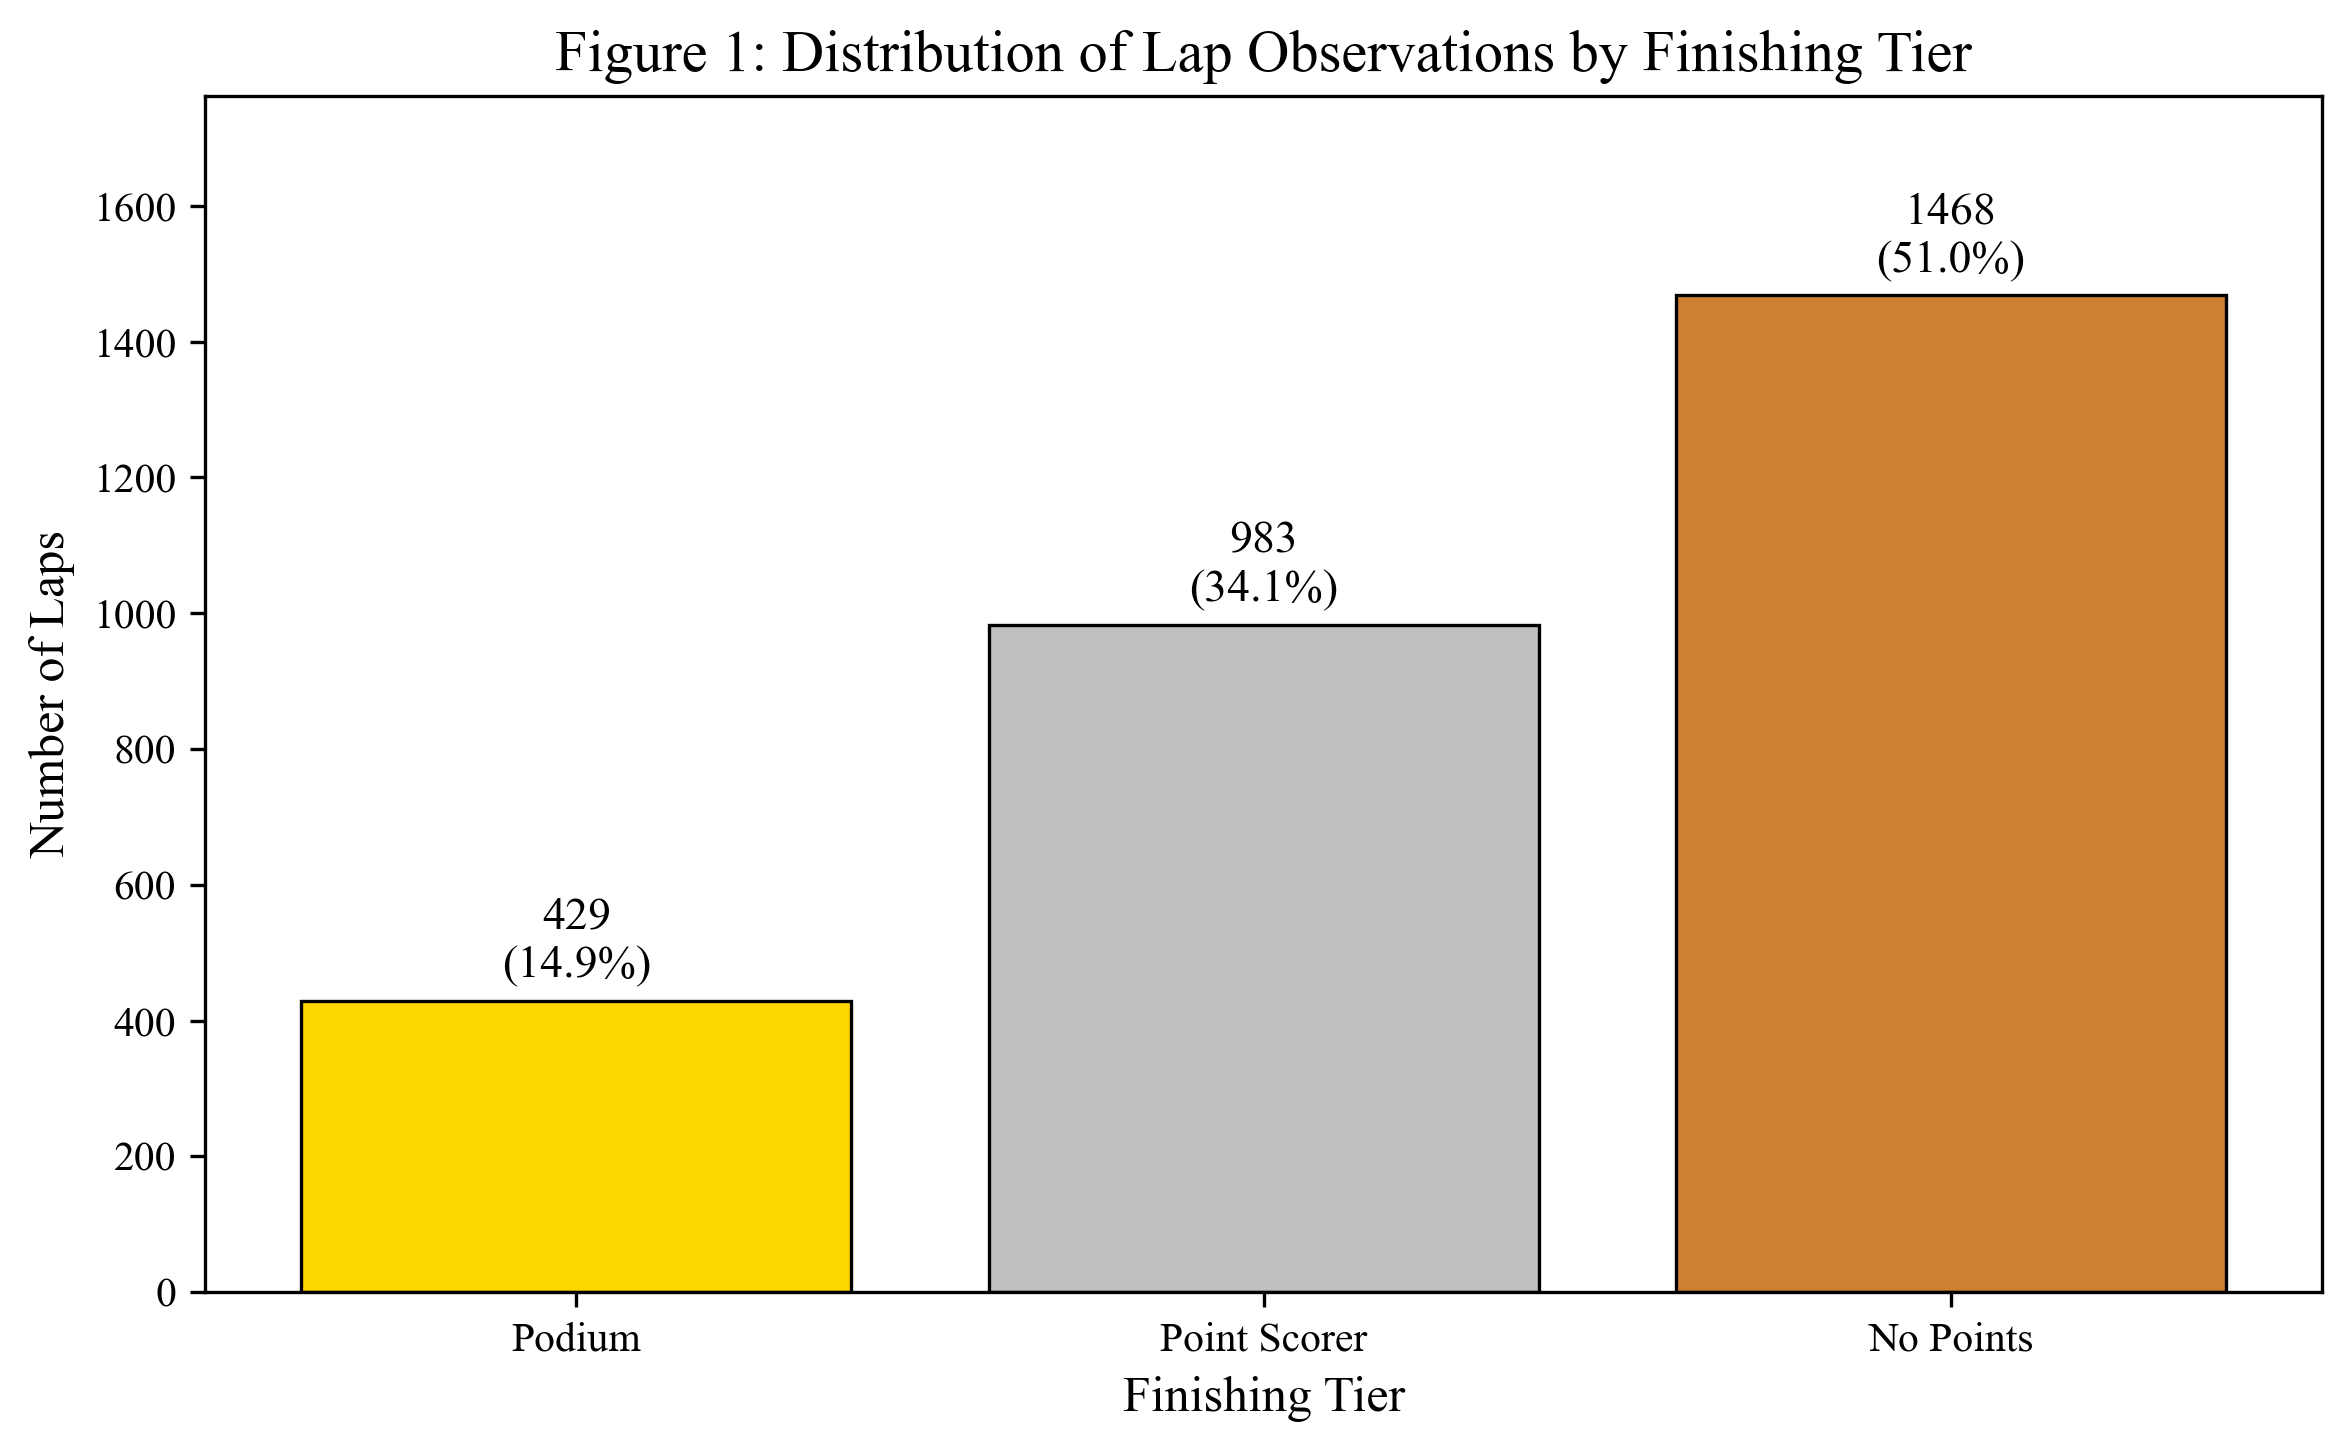
\includegraphics[width=0.75\textwidth]{figures/fig1_class_distribution.png}
  \caption{Distribution of Lap Observations by Finishing Tier}
  \label{fig:class-dist}
\end{figure}

\noindent
The ``No Points'' tier accounts for 50.97\% of all laps, ``Point Scorer''
for 34.13\%, and ``Podium'' for 14.90\%. This imbalance reflects the
real-world structure of Formula One: only three of twenty drivers finish on
the podium, while the majority of the field competes for positions outside
the points. The class imbalance was addressed during machine learning
validation through balanced class weighting.

\subsection{Box's M Test: Homogeneity of Covariance Matrices}

Box's M test was conducted to determine whether the variance--covariance
matrices of the continuous predictors were equal across the three finishing
tiers.

\begin{table}[htbp]
  \centering
  \caption{Box's M Test Results}
  \label{tab:boxs-m}
  \begin{tabular}{lc}
    \toprule
    \textbf{Statistic} & \textbf{Value} \\
    \midrule
    Chi-square (approx.) & 160.419 \\
    Degrees of freedom   & 20 \\
    $p$-value            & $< 2.2 \times 10^{-16}$ \\
    \bottomrule
  \end{tabular}
\end{table}

The test yielded $\chi^{2}(20) = 160.419$, $p < 2.2 \times 10^{-16}$,
decisively rejecting the null hypothesis of equal covariance matrices. This
result has a direct methodological consequence: Multiple Discriminant Analysis
(MDA) requires homogeneous covariance structures for valid classification.
Because this assumption is violated, MDA is disqualified and
\textbf{multinomial logistic regression} was adopted as the primary
inferential model. Unlike MDA, multinomial logistic regression makes no
assumption about the covariance structure across groups---it estimates
separate log-odds equations for each non-baseline category without requiring
pooled covariance.

\subsection{VIF Diagnostics: Multicollinearity Check}

Variance inflation factors were computed for all predictors to ensure that
the engineered features---particularly the interaction term and its component
variables---did not introduce problematic multicollinearity.

\begin{table}[htbp]
  \centering
  \caption{Variance Inflation Factor (VIF) Diagnostics}
  \label{tab:vif}
  \begin{tabular}{lc}
    \toprule
    \textbf{Variable} & \textbf{VIF} \\
    \midrule
    GridPosition         & 1.007 \\
    Tire\_Age            & 3.220 \\
    Fuel\_Mass\_Proxy    & 2.315 \\
    Degradation\_x\_Fuel & 1.725 \\
    Tire\_MEDIUM         & 1.181 \\
    Tire\_SOFT           & 1.156 \\
    \bottomrule
  \end{tabular}
\end{table}

\begin{figure}[htbp]
  \centering
  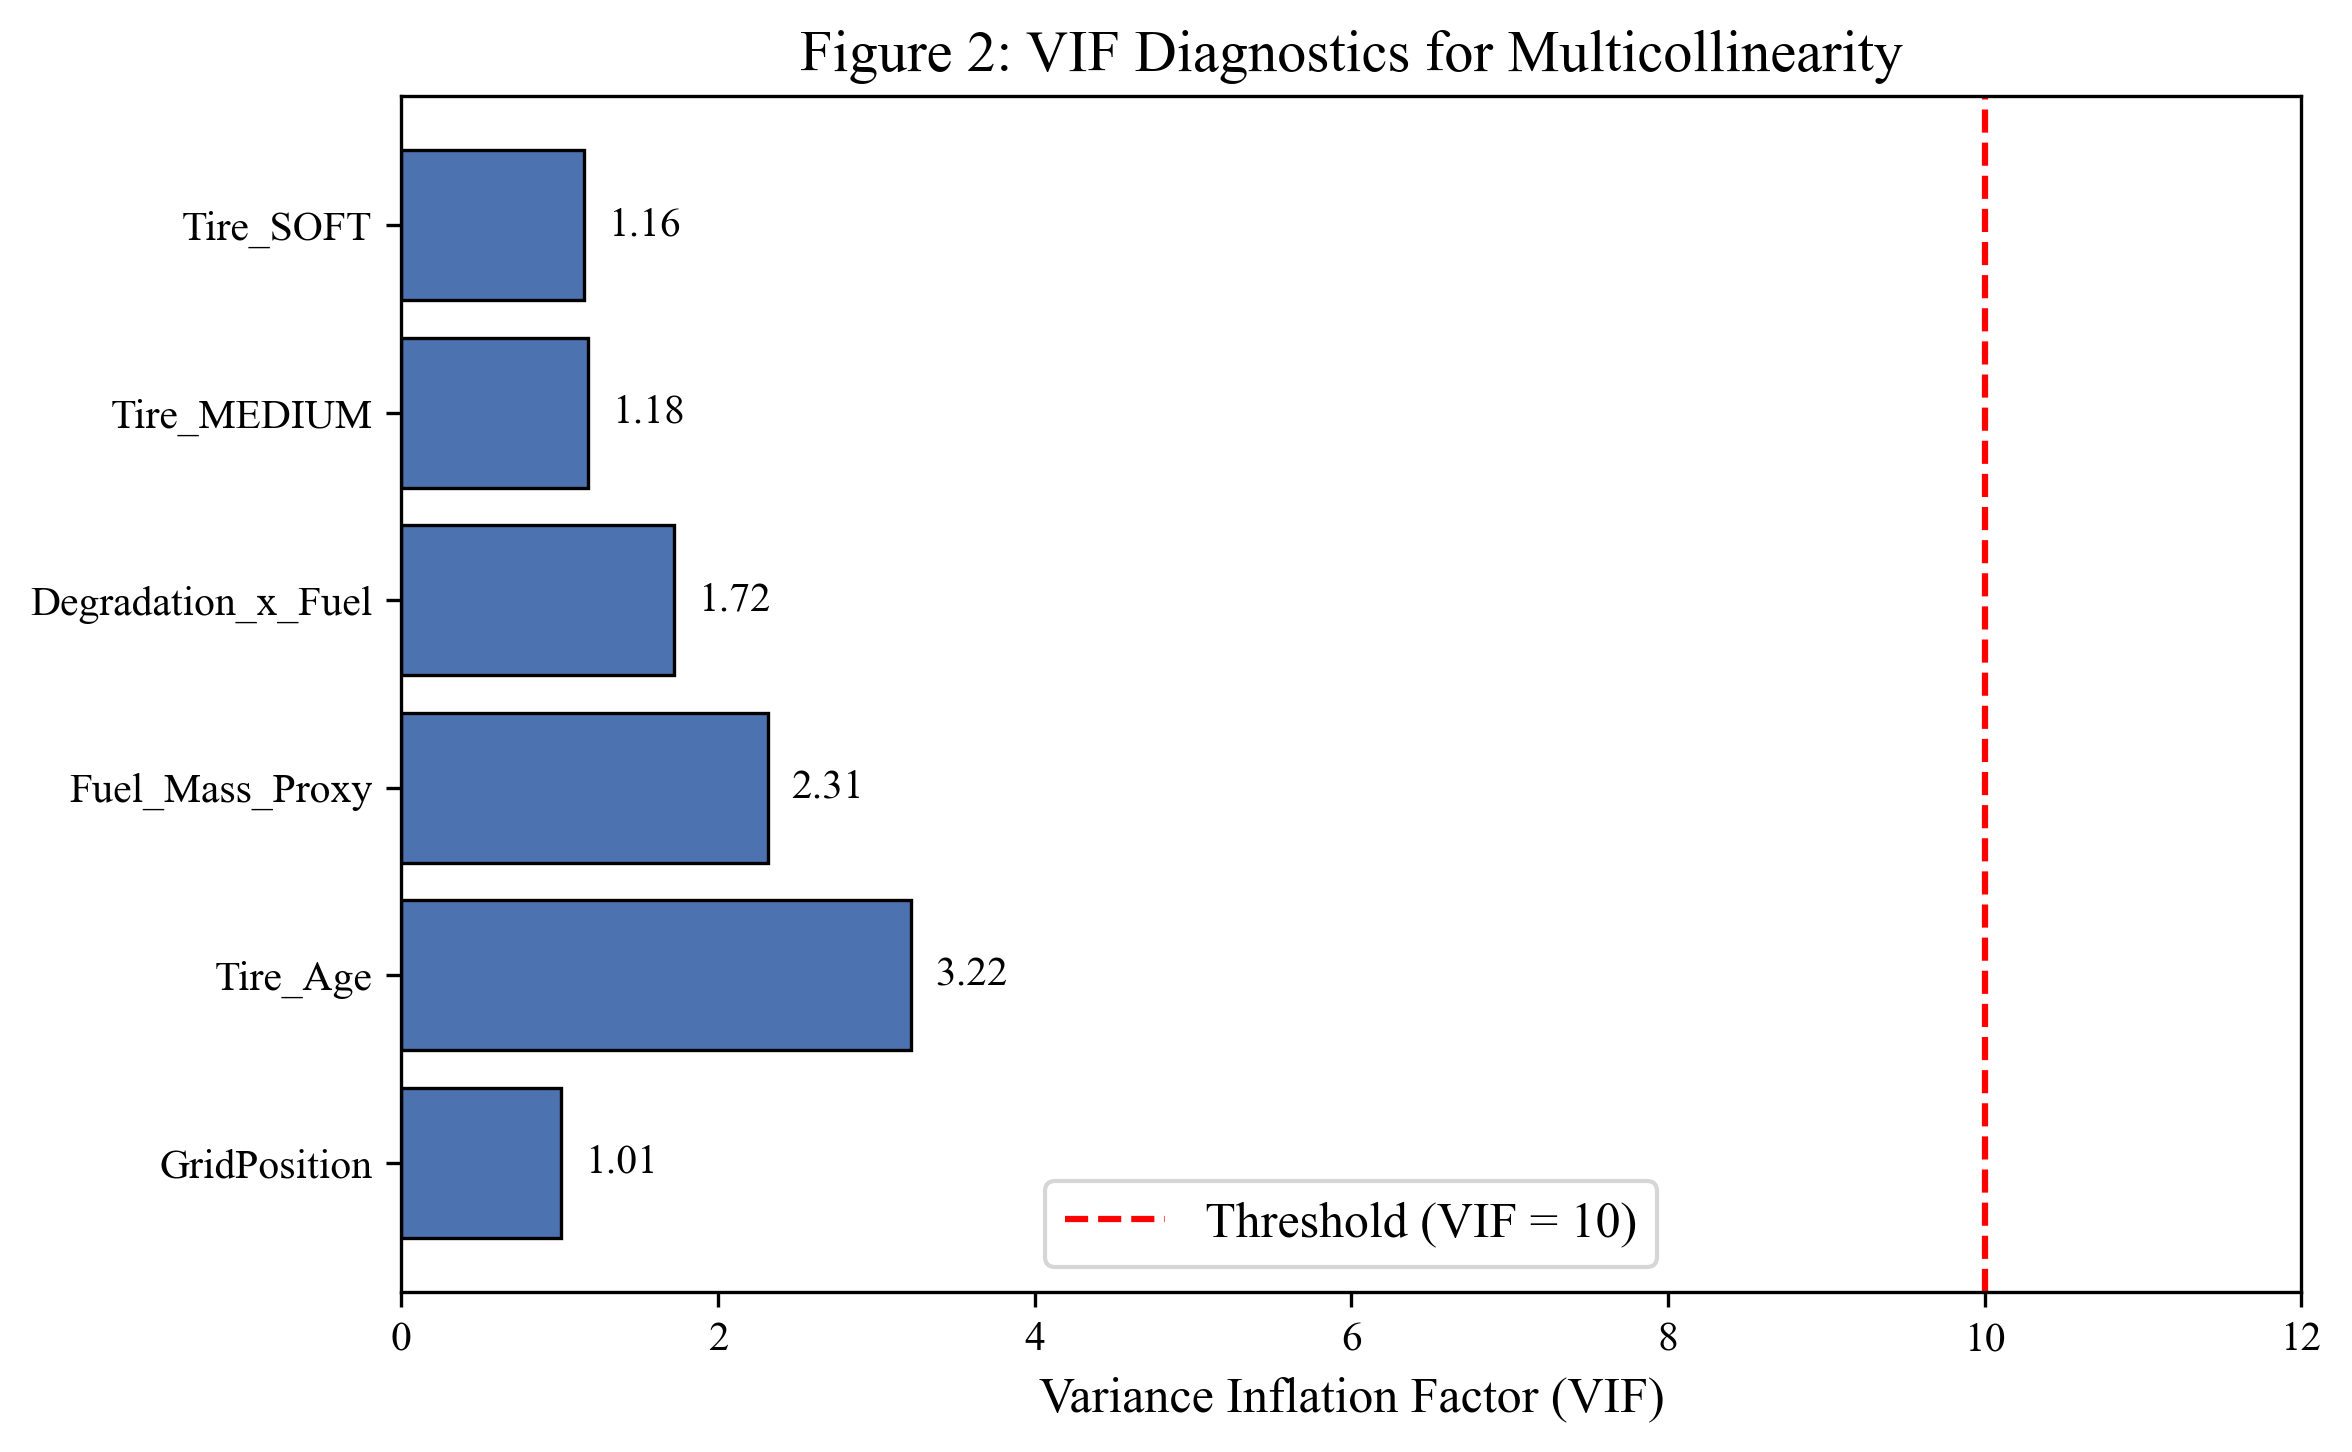
\includegraphics[width=0.75\textwidth]{figures/fig2_vif.png}
  \caption{VIF Diagnostics for Multicollinearity (threshold = 10)}
  \label{fig:vif}
\end{figure}

All VIF values fall well below the standard threshold of 10 (Table~\ref{tab:vif},
Figure~\ref{fig:vif}). The highest value is 3.22 for Tire\_Age, which is
within acceptable limits and reflects a moderate correlation with Fuel\_Mass\_Proxy
(VIF = 2.32)---an expected physical relationship since both variables increase
monotonically with race distance.

Critically, the Degradation $\times$ Fuel interaction term registers a VIF
of only 1.725, confirming that the mean-centering procedure effectively
eliminated structural multicollinearity. Without mean-centering, the product
of two correlated variables would inherit and amplify their correlation,
inflating standard errors and destabilizing coefficient estimates.

The near-perfect VIF of 1.007 for GridPosition confirms that starting
position and within-race telemetry are statistically independent---a finding
that is physically expected since grid position is determined in qualifying
(over a single flying lap) while tire age and fuel mass accumulate during
the race.

\subsection{Multinomial Logistic Regression (MLE)}

The multinomial logistic regression model was fitted with ``No Points'' as the
baseline category. All coefficients represent log-odds relative to this
reference tier.

\subsubsection{Model Fit Statistics}

\begin{table}[htbp]
  \centering
  \caption{Multinomial Logistic Regression Model Fit}
  \label{tab:model-fit}
  \begin{tabular}{lc}
    \toprule
    \textbf{Statistic} & \textbf{Value} \\
    \midrule
    Residual Deviance & 3821.657 \\
    AIC               & 3849.657 \\
    Observations      & 2,880 \\
    Predictors        & 6 \\
    Response Classes  & 3 \\
    \bottomrule
  \end{tabular}
\end{table}

\subsubsection{Coefficient Estimates and Significance}

\begin{table}[htbp]
  \centering
  \caption{MLE Coefficient Estimates (Log-Odds)}
  \label{tab:coefficients}
  \small
  \begin{tabular}{lrr}
    \toprule
    \textbf{Predictor} & \textbf{Podium} & \textbf{Point Scorer} \\
    \midrule
    Intercept            &  4.8565  &  2.9230 \\
    GridPosition         & $-0.7978$ & $-0.2271$ \\
    Tire\_Age            &  0.0291  & $-0.0036$ \\
    Fuel\_Mass\_Proxy    & $-0.0149$ & $-0.0084$ \\
    Degradation\_x\_Fuel &  0.0008  &  0.0002 \\
    Tire\_MEDIUM         &  0.2267  & $-0.4601$ \\
    Tire\_SOFT           &  0.2424  & $-0.2538$ \\
    \bottomrule
  \end{tabular}
\end{table}

\begin{table}[htbp]
  \centering
  \caption{Standard Errors of Coefficient Estimates}
  \label{tab:std-errors}
  \small
  \begin{tabular}{lrr}
    \toprule
    \textbf{Predictor} & \textbf{Podium} & \textbf{Point Scorer} \\
    \midrule
    Intercept            & 0.4206  & 0.2511 \\
    GridPosition         & 0.0347  & 0.0107 \\
    Tire\_Age            & 0.0136  & 0.0075 \\
    Fuel\_Mass\_Proxy    & 0.0045  & 0.0023 \\
    Degradation\_x\_Fuel & 0.0003  & 0.0002 \\
    Tire\_MEDIUM         & 0.2628  & 0.1376 \\
    Tire\_SOFT           & 0.2740  & 0.1317 \\
    \bottomrule
  \end{tabular}
\end{table}

\begin{table}[htbp]
  \centering
  \caption{$p$-Values for Coefficient Significance}
  \label{tab:pvalues}
  \small
  \begin{tabular}{lrr}
    \toprule
    \textbf{Predictor} & \textbf{Podium} & \textbf{Point Scorer} \\
    \midrule
    Intercept            & 0.0000 & 0.0000 \\
    GridPosition         & 0.0000 & 0.0000 \\
    Tire\_Age            & 0.0328 & 0.6337 \\
    Fuel\_Mass\_Proxy    & 0.0009 & 0.0003 \\
    Degradation\_x\_Fuel & 0.0095 & 0.2174 \\
    Tire\_MEDIUM         & 0.3883 & 0.0008 \\
    Tire\_SOFT           & 0.3764 & 0.0540 \\
    \bottomrule
  \end{tabular}
\end{table}

\begin{figure}[htbp]
  \centering
  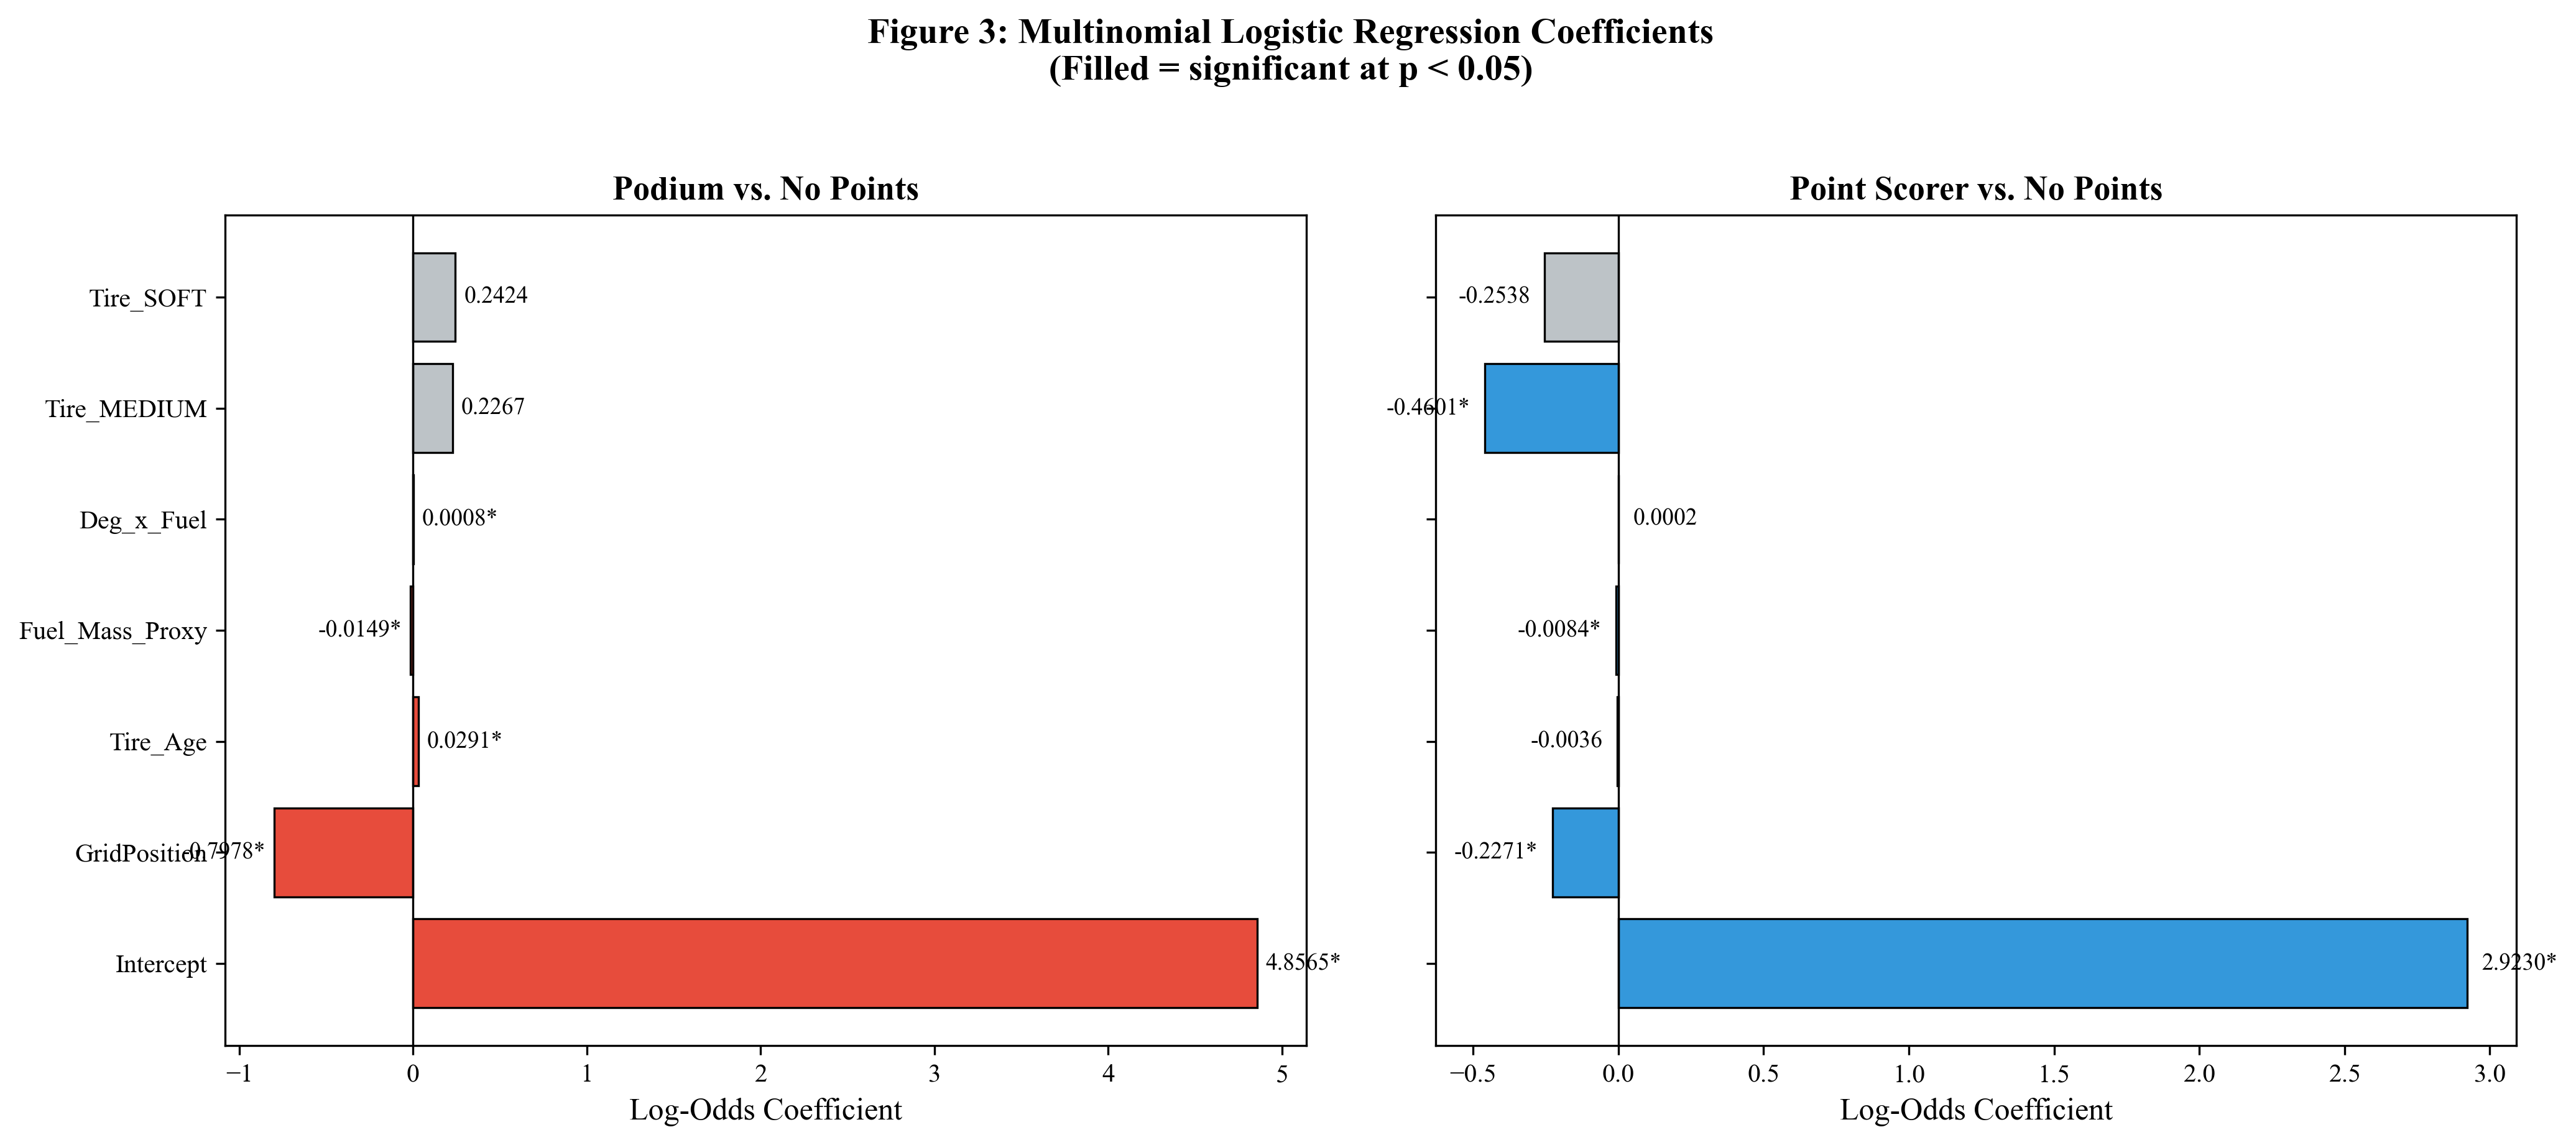
\includegraphics[width=\textwidth]{figures/fig3_coefficients.png}
  \caption{MLE Coefficients by Tier (filled bars = significant at $p < 0.05$)}
  \label{fig:coefficients}
\end{figure}

\subsubsection{Interpretation of Key Findings}

Figure~\ref{fig:coefficients} visualizes the coefficient estimates, with
filled bars indicating statistical significance at $\alpha = 0.05$.

\paragraph{GridPosition ($p = 0.000$ for both tiers).}
Starting position is overwhelmingly significant for both the Podium and Point
Scorer tiers. The coefficient of $-0.80$ for Podium means that each position
further back on the grid reduces the log-odds of a podium finish by
approximately 0.80 units. In odds-ratio terms, moving back one grid position
multiplies the odds of a podium finish by $e^{-0.80} \approx 0.45$---a
55\% reduction per grid slot. This is the dominant predictor in the model and
confirms the well-known difficulty of overtaking in modern F1.

\paragraph{Degradation $\times$ Fuel ($p = 0.0095$ for Podium).}
With grid position controlling for raw car pace, the interaction term achieves
significance at $\alpha < 0.01$ for the Podium tier. The positive coefficient
(0.0008) indicates that when tire age and fuel mass are both high---i.e.,
early-race conditions where the car is heavy and tires are relatively
fresh---the combined physical effect favors podium outcomes. This is
mechanistically consistent: top-tier teams and drivers manage tire degradation
more effectively under heavy fuel loads, maintaining competitive lap times
while midfield competitors lose performance to the combined stress of mass
and rubber wear.

\paragraph{Fuel\_Mass\_Proxy ($p = 0.0009$ Podium, $p = 0.0003$ Point Scorer).}
Fuel mass is significant for both tiers. The negative coefficients mean that
as fuel burns off (decreasing mass), the log-odds of being in the Podium or
Point Scorer tier increase relative to No Points. This reflects the physical
reality that lighter cars are faster---but since fuel mass decreases
monotonically with lap number, this variable also partially captures the
effect of race progression.

\paragraph{Tire\_MEDIUM ($p = 0.0008$ for Point Scorer).}
Medium tire compound is significant for the Point Scorer tier with a negative
coefficient ($-0.46$), indicating that laps on medium tires are associated
with lower log-odds of being in the Point Scorer tier relative to the Hard
baseline. This likely reflects strategic patterns: top teams often start on
Softs and switch to Hards, while midfield teams rely more heavily on Mediums.

\paragraph{Non-significant predictors.}
Tire\_SOFT ($p = 0.3764$ Podium, $p = 0.0540$ Point Scorer) and
Tire\_MEDIUM for Podium ($p = 0.3883$) do not reach significance. This
suggests that compound choice alone, independent of how the tire degrades
over its stint, does not differentiate podium performers from the baseline.

\subsection{Grid Position and Finishing Tier}

Figure~\ref{fig:grid-box} shows the distribution of grid positions across
finishing tiers, providing visual confirmation of GridPosition's predictive
power.

\begin{figure}[htbp]
  \centering
  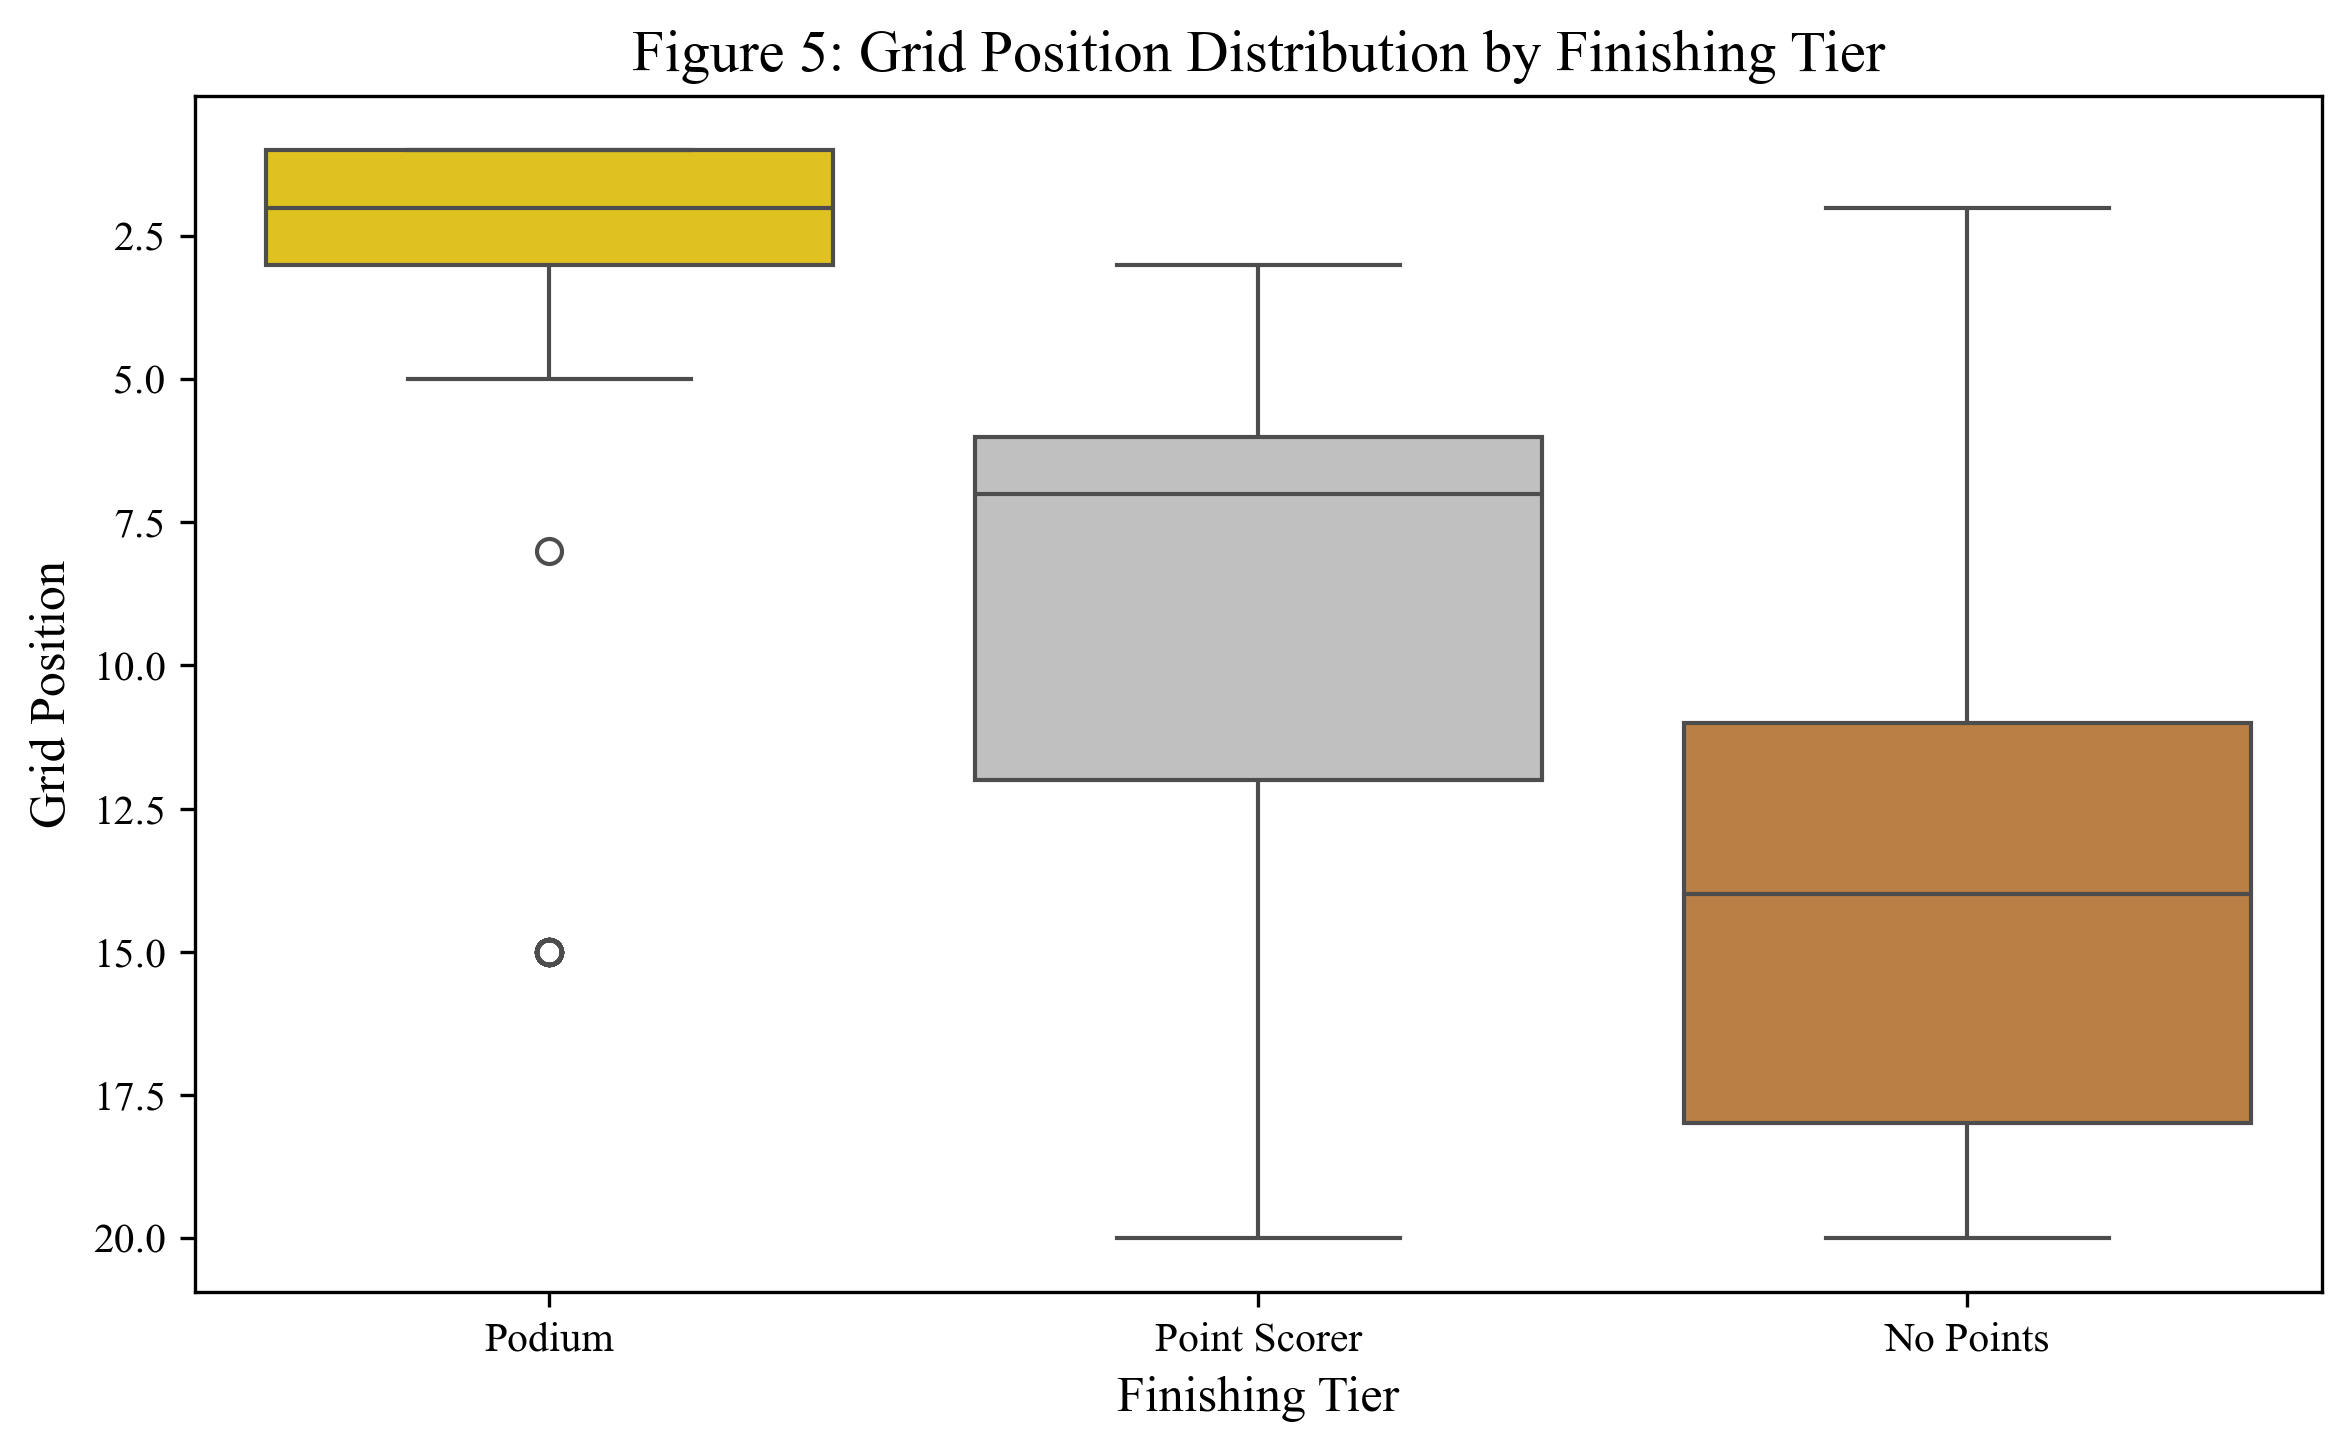
\includegraphics[width=0.75\textwidth]{figures/fig5_gridposition_boxplot.png}
  \caption{Grid Position Distribution by Finishing Tier}
  \label{fig:grid-box}
\end{figure}

Podium finishers cluster at grid positions 1--5 with a tight interquartile
range, while No Points finishers span positions 8--20 with substantial
variance. Point Scorers occupy the middle ground (positions 4--12). The
minimal overlap between Podium and No Points boxes confirms why
GridPosition achieves such high statistical significance.

\subsection{Tire Age vs.\ Fuel Mass by Tier}

Figure~\ref{fig:scatter} visualizes the two primary telemetry features
across all three tiers, revealing the physical clustering patterns the model
captures.

\begin{figure}[htbp]
  \centering
  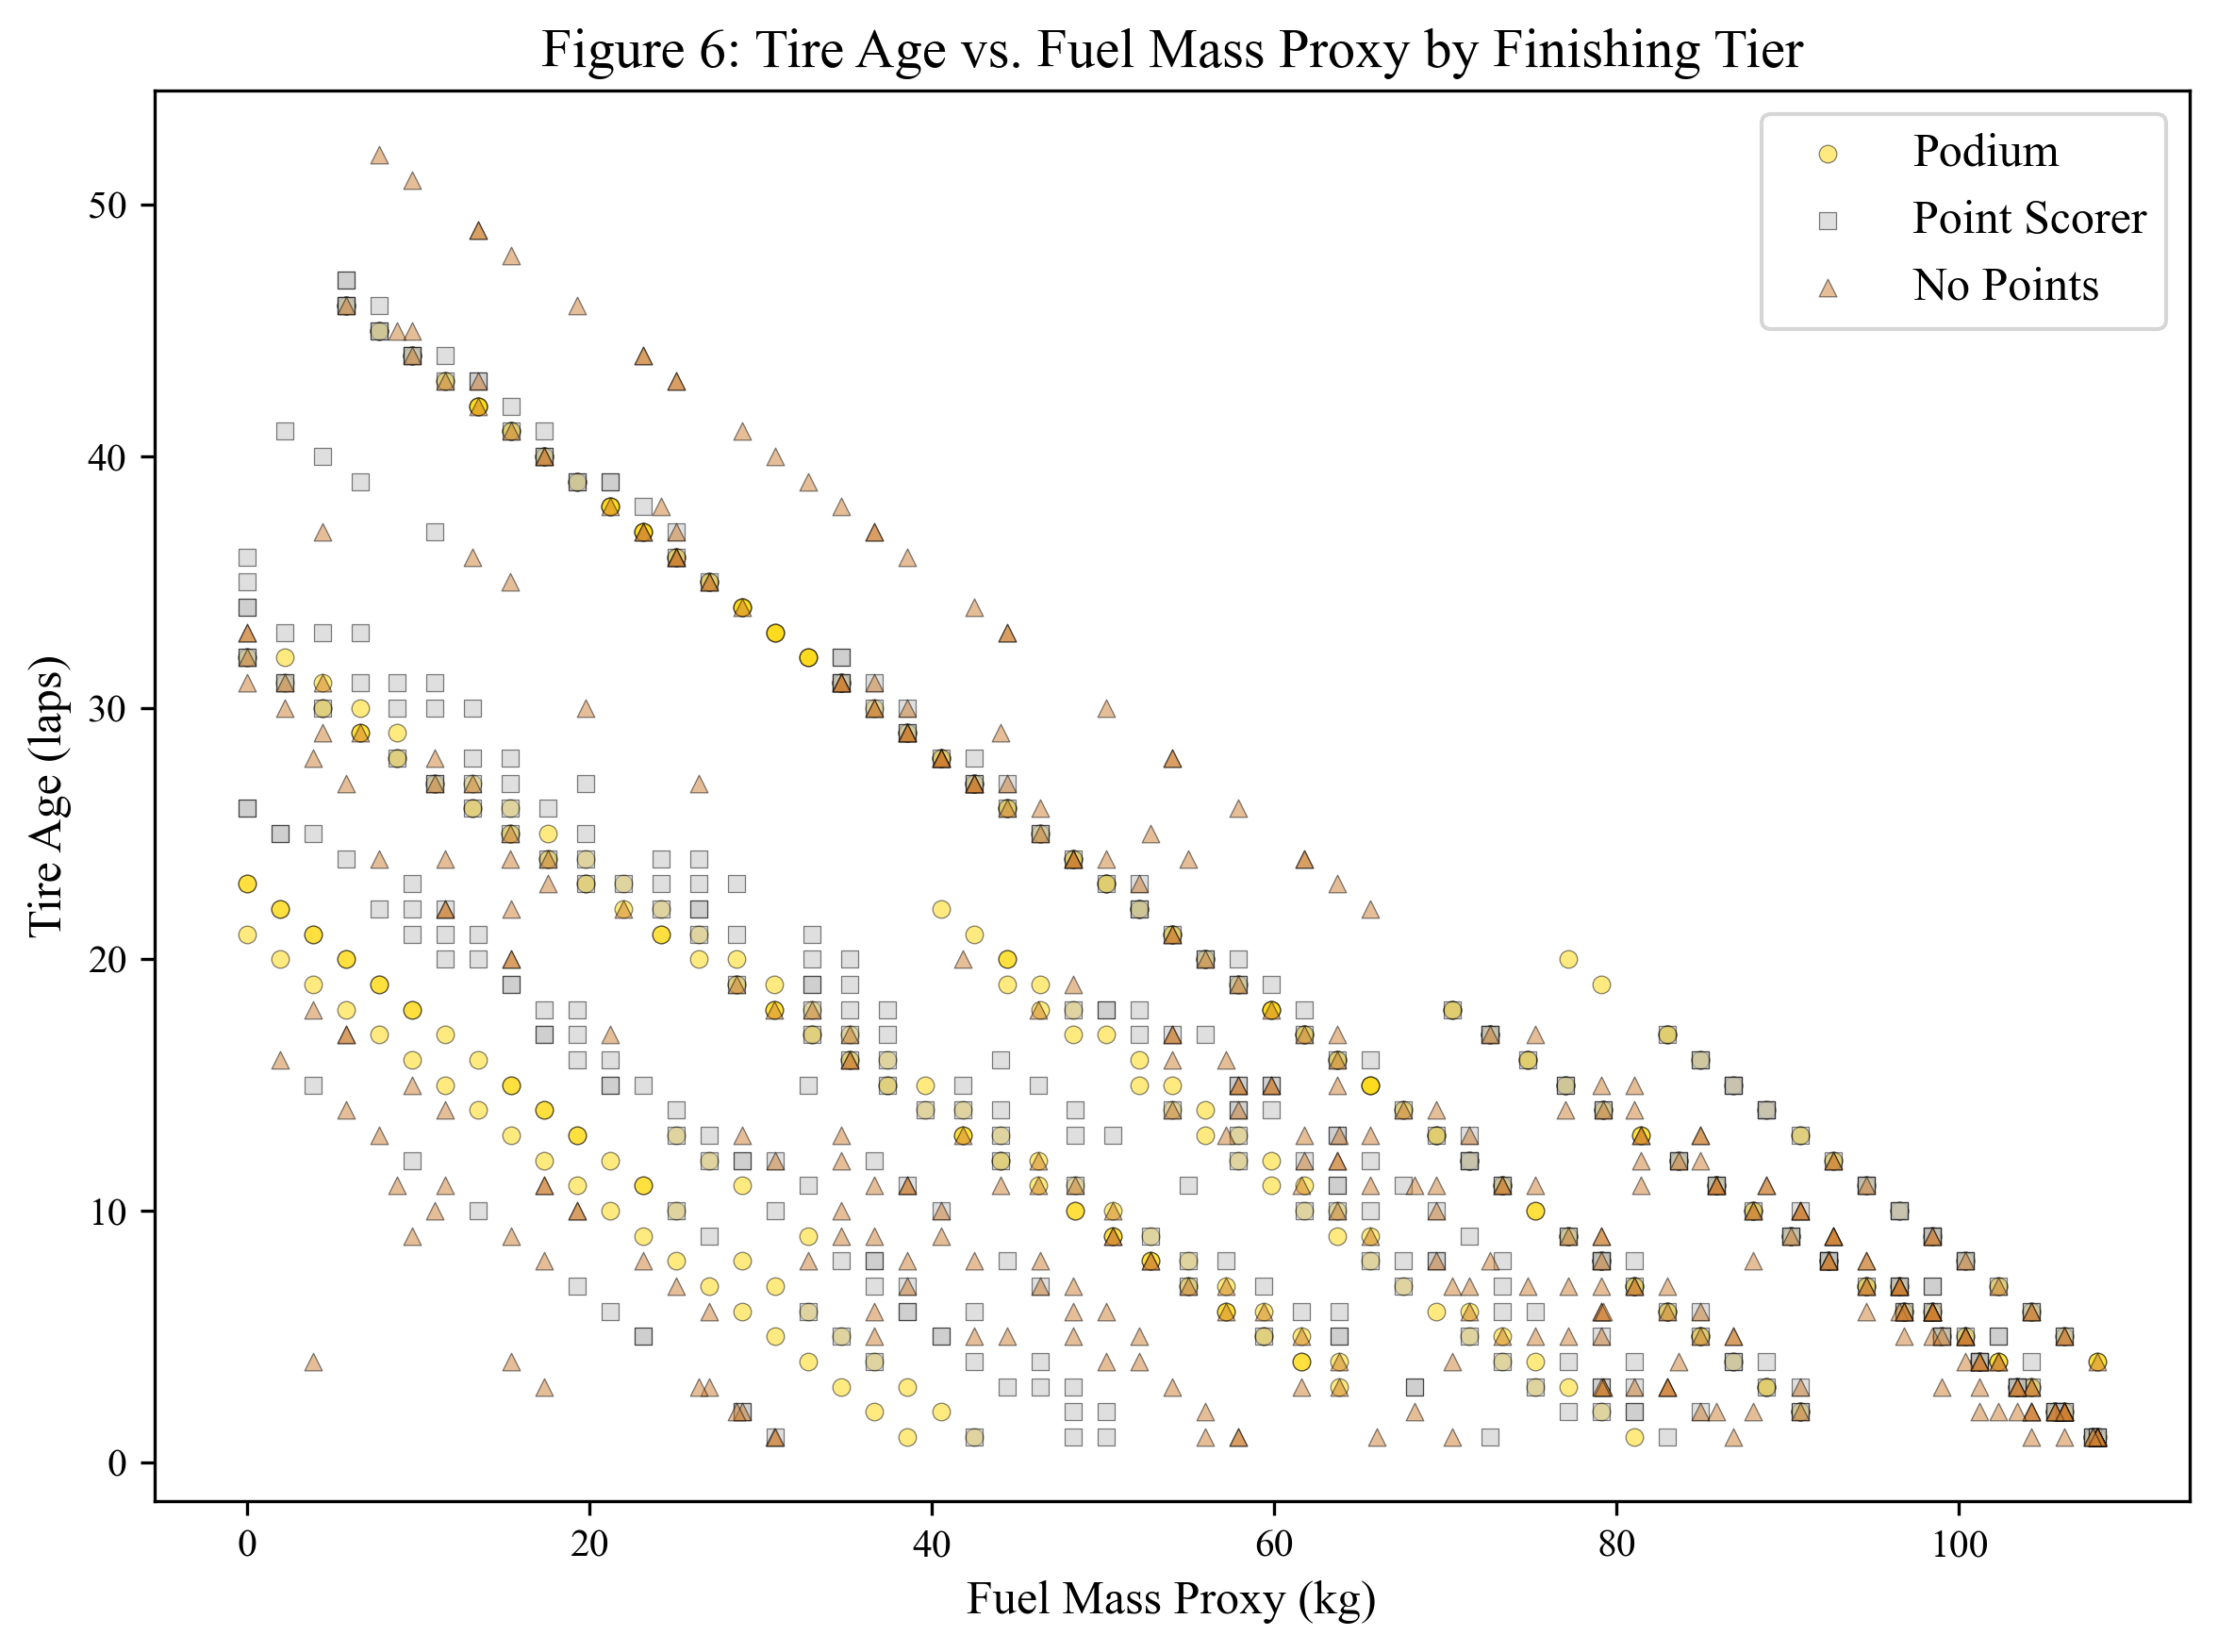
\includegraphics[width=0.8\textwidth]{figures/fig6_scatter_tierfuel.png}
  \caption{Tire Age vs.\ Fuel Mass Proxy by Finishing Tier}
  \label{fig:scatter}
\end{figure}

The scatter plot shows that Podium laps (gold) are concentrated in the
low--tire-age, high--fuel-mass region (early race, fresh tires) and the
high--tire-age, low--fuel-mass region (late race, light car on worn tires).
No Points laps (bronze) are more uniformly distributed. The interaction term
captures the diagonal structure where these two forces combine differently
across the race timeline.

\subsection{Machine Learning Validation (LOGO-CV)}

To test whether the statistical equation generalizes to unseen circuits, a
multinomial logistic regression with balanced class weighting was validated
using leave-one-group-out cross-validation across the three races.


\subsubsection{Classification Performance}

\begin{table}[H]
  \centering
  \caption{LOGO-CV Classification Report}
  \label{tab:classification}
  \begin{tabular}{lcccc}
    \toprule
    \textbf{Tier} & \textbf{Precision} & \textbf{Recall} &
    \textbf{F1-Score} & \textbf{Support} \\
    \midrule
    No Points     & 0.74 & 0.67 & 0.70 & 1,468 \\
    Podium        & 0.57 & 0.89 & 0.69 & 429 \\
    Point Scorer  & 0.49 & 0.45 & 0.47 & 983 \\
    \midrule
    \multicolumn{4}{l}{\textbf{Overall Accuracy}} & \textbf{62.36\%} \\
    \bottomrule
  \end{tabular}
\end{table}

\begin{figure}[H]
  \centering
  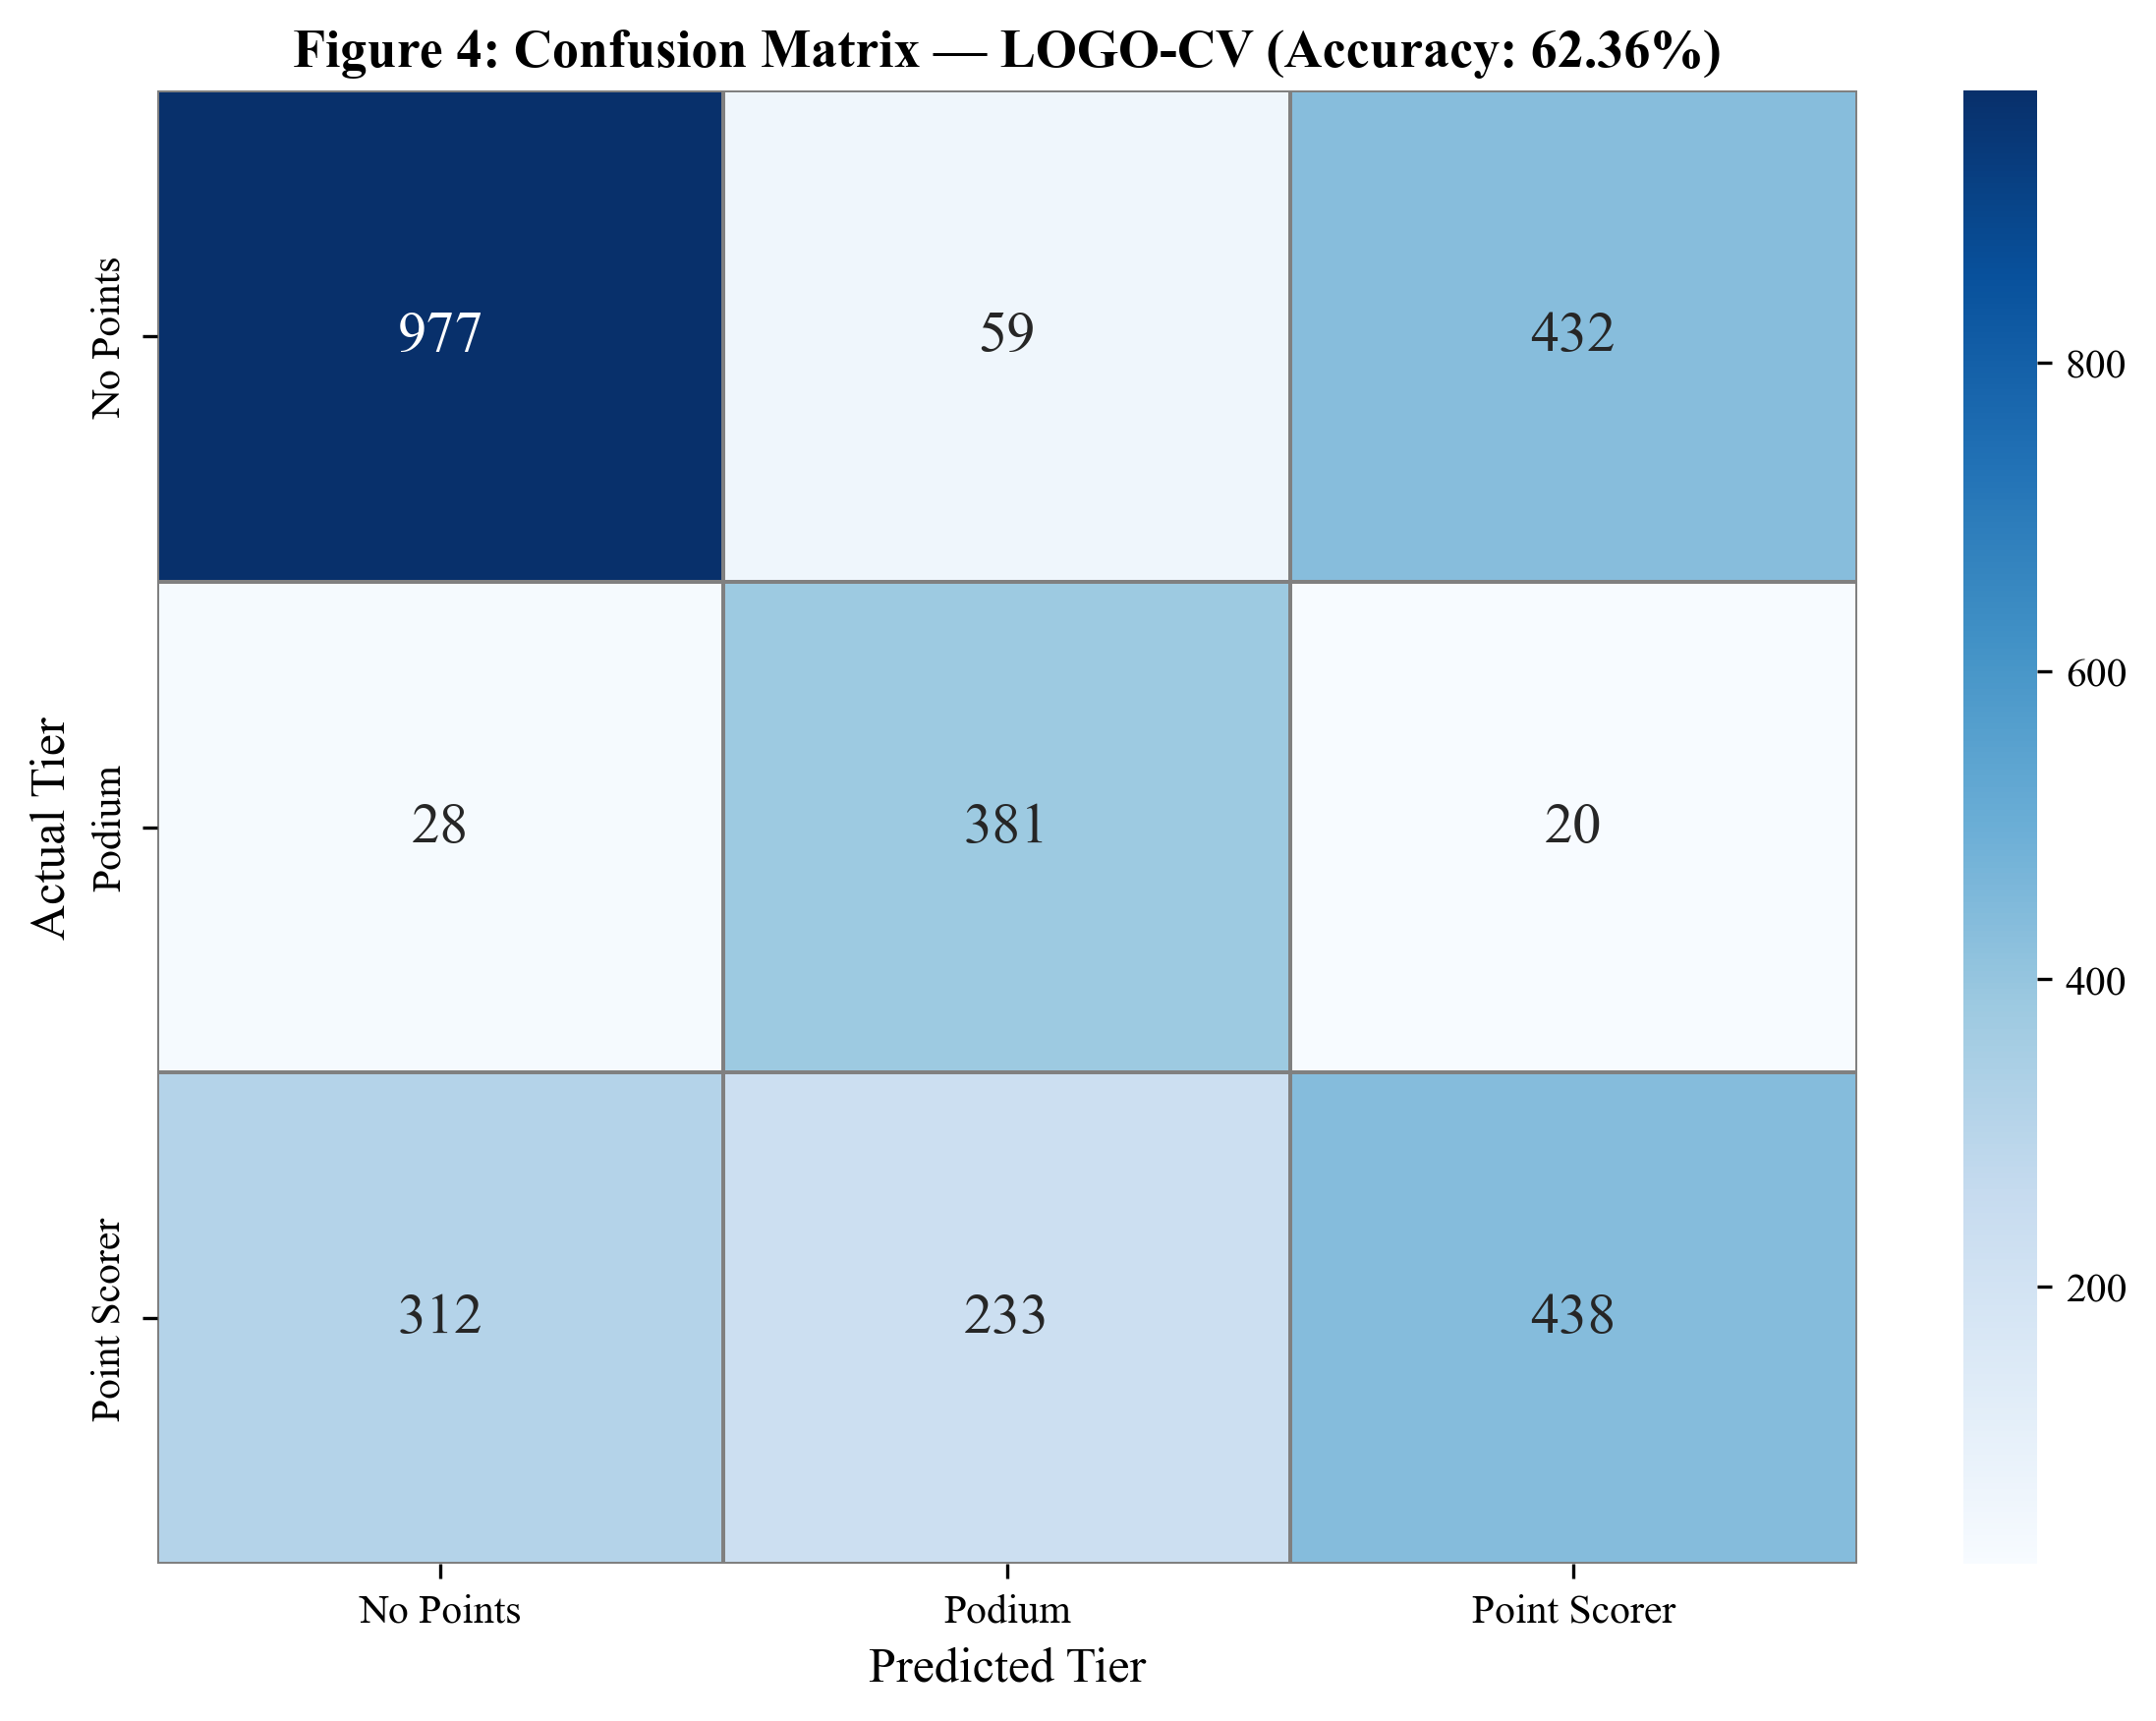
\includegraphics[width=0.75\textwidth]{figures/fig4_confusion_matrix.png}
  \caption{Confusion Matrix from LOGO-CV}
  \label{fig:confusion}
\end{figure}

\subsubsection{Interpretation}

\textbf{Podium recall (0.89).} The model correctly identified 89\% of all
actual podium-finishing laps across held-out circuits. This is the strongest
result in the validation and demonstrates that the combination of grid
position control and telemetry-based features captures top-tier performance
signatures reliably---even when the model has never seen that circuit's data.

\textbf{Podium precision (0.57).} Of all laps the model predicted as
``Podium,'' 57\% were correct. The 43\% false positive rate consists
primarily of Point Scorer laps misclassified as Podium---an understandable
error given that positions 4--6 often run similar pace to P3.

\textbf{No Points performance (Precision = 0.74, Recall = 0.67).} The
model is most precise when identifying No Points laps, correctly flagging
74\% of its predictions for this class. The 33\% miss rate reflects the
reality that some drivers in backmarker grid positions produce strong
individual laps (e.g., during low-fuel late stints) that the model
temporarily classifies as Point Scorer pace.

\textbf{Point Scorer recall (0.45).} The model caught only 45\% of
point-scoring laps. The F1 midfield is genuinely harder to model---DRS
trains create artificial pace spikes, undercut strategies shuffle the order
independently of telemetry, and intra-team race orders can suppress or
inflate individual lap times. The confusion matrix (Figure~\ref{fig:confusion})
shows that most Point Scorer errors split between Podium (over-prediction)
and No Points (under-prediction), confirming this tier sits at the decision
boundary.

\textbf{Overall accuracy (62.36\%).} For a three-class problem with natural
class imbalance and strict cross-circuit validation (no data leakage), this
substantially outperforms random guessing (33.3\%) and majority-class
prediction (51.0\%). More importantly, the LOGO-CV design ensures this is an
honest estimate of out-of-sample performance---the model cannot memorize
circuit-specific patterns because each fold tests on a completely unseen
race.
